\section{if-conversion的执行策略}

\subsection{if-conversion给编译器带来的挑战}

1997年,August在文章中详细讨论了处理器对谓词执行的支持给编译器带来的挑战,以及if-conversion的研究需要解决的问题\cite{August1997}。现将August的分析总结如下:



\subsection{August的基于逆向if-conversion的平衡算法}

August建议,在编译过程的早期大量应用if-conversion来发掘谓词执行带来的全部好处,此时形成的Hyperblock比目标体系能处理的大得多,然后在比较靠后的编译阶段进行部分逆向if-conversion,根据目标机器调整每个Hyperblock的谓词化代码的数量,以平衡控制流跟谓词数目。整个过程的工作流程如\fref{fig:ifcvtframework}所示。

\begin{figure}
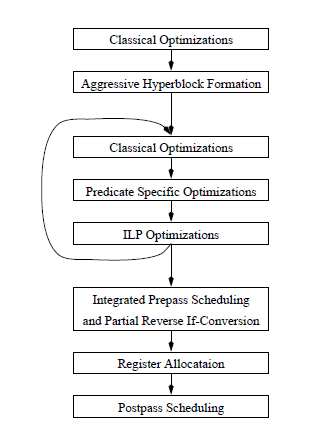
\includegraphics[width=\linewidth]{ifcvt-framework}
\caption{\label{fig:ifcvtframework} if-conversion的执行策略}
\end{figure}
